% slides/05_preprocessing.tex


\begin{frame}{Flujo de trabajo de preprocesamiento en qEEG}
  \begin{columns}[T]
    \begin{column}{0.52\textwidth}
      \textbf{Procesos comunes}
      \begin{enumerate}
        \item Cambio de referencia (CAR / REST)
        \item Filtrado pasa/rechaza banda
        \item Segmentación basada en tiempo o en marcas
        \item Rechazo/interpolación de épocas 
        \item Artifact subspace reconstruction (ASR) \cite{Mullen2015}
        \item Descomposición y clasificación de componentes ICA (ICLabel) \cite{PionTonachini2019}
      \end{enumerate}
    \end{column}
    \begin{column}{0.45\textwidth}
      \begin{alertblock}{Matriz de confusión ICLabel}
      	\begin{center}
        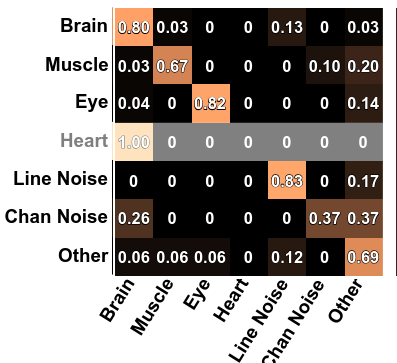
\includegraphics[width=0.7\textwidth]{imagenes/iclabel.png}
        \end{center}
      \end{alertblock}
    \end{column}
  \end{columns}
\end{frame}
